\chapter{GNU Emacs et ESS: la base}
\label{emacs+ess}

Emacs est l'Éditeur de texte des éditeurs de texte. Conçu à l'origine
comme un éditeur pour les programmeurs (avec des modes spéciaux pour
une multitude de langages différents), Emacs est devenu au fil du
temps un environnement logiciel en soi dans lequel on peut réaliser
une foule de tâches différentes: rédiger des documents \LaTeX,
interagir avec R, SAS ou un logiciel de base de données, consulter son
courrier électronique, gérer son calendrier ou même jouer à Tetris!

Cette annexe passe en revue les quelques commandes essentielles à
connaître pour commencer à travailler avec GNU Emacs et le mode ESS.
L'ouvrage de \cite{Cameron:Emacs:2004} constitue une excellente
référence pour l'apprentissage plus poussé de l'éditeur.


\section{Mise en contexte}
\label{emacs+ess:contexte}

Emacs est le logiciel étendard du projet GNU («\emph{GNU is not
  Unix}»), dont le principal commanditaire est la \emph{Free Software
  Foundation} (FSF) à l'origine de tout le mouvement du logiciel
libre.
\begin{itemize}
\item Richard M.\ Stallman, président de la FSF et grand apôtre du
  libre, a écrit la première version de Emacs et il continue à ce jour
  à contribuer au projet.
\item Les origines de Emacs remontent au début des années 1980, une
  époque où les interfaces graphiques n'existaient pas, le parc
  informatique était beaucoup plus hétérogène qu'aujourd'hui (les
  claviers n'étaient pas les mêmes d'une marque d'ordinateur à une
  autre) et les modes de communication entre les ordinateurs
  demeuraient rudimentaires.
\item L'âge vénérable de Emacs transparaît à plusieurs endroits,
  notamment dans la terminologie inhabituelle, les raccourcis clavier
  non conformes aux standards d'aujourd'hui ou la manipulation des
  fenêtres qui ne se fait pas avec une souris.
\end{itemize}

Emacs s'adapte à différentes tâches par l'entremise de \emph{modes}
qui modifient son comportement ou lui ajoutent des fonctionnalités.
L'un de ces modes est ESS (\emph{Emacs Speaks Statistics}).
\begin{itemize}
\item ESS permet d'interagir avec des logiciels statistiques (en
  particulier R, S+ et SAS) directement depuis Emacs.
\item Quelques-uns des développeurs de ESS sont aussi des développeurs
  de R, d'où la grande compatibilité entre les deux logiciels.
\item Lorsque ESS est installé, le mode est activé automatiquement en
  ouvrant dans Emacs un fichier dont le nom se termine par l'extension
  \code{.R}.
\end{itemize}


\section{Installation}
\label{emacs+ess:installation}

GNU Emacs et le mode ESS sont normalement livrés d'office avec toutes
les distributions Linux. Pour les environnements Windows et Mac OS~X,
le plus simple consiste à télécharger et installer les distributions
préparées par le présent auteur. Consulter le site
\begin{quote}
  \url{http://vgoulet.act.ulaval.ca/emacs/}
\end{quote}


\section{Description sommaire}
\label{emacs+ess:description}

Au lancement, Emacs affiche un écran d'information contenant des liens
vers différentes ressources. Cet écran disparaît dès que l'on appuie
sur une touche. La fenêtre Emacs se divise en quatre zone principales
(voir la \autoref{fig:ess:emacswindow}):
\begin{enumerate}
\item tout au haut de la fenêtre (ou de l'écran sous OS~X), on trouve
  l'habituelle barre de menu dont le contenu change selon le mode dans
  lequel se trouve Emacs;
\item l'essentiel de la fenêtre sert à afficher un \emph{buffer}, soit
  le contenu d'un fichier ouvert ou l'invite de commande d'un
  programme externe;
\item la ligne de mode est le séparateur horizontal contenant diverses
  informations sur le fichier ouvert et l'état de Emacs;
\item le \emph{minibuffer} est la région au bas de la fenêtre où l'on
  entre des commandes et reçoit de l'information de Emacs.
\end{enumerate}
Il est possible de séparer la fenêtre Emacs en sous-fenêtres pour
afficher plusieurs \emph{buffers} à la fois. Il y a alors une ligne de
mode pour chaque \emph{buffer}.

\begin{figure}[t]
  %% Capture d'écran
  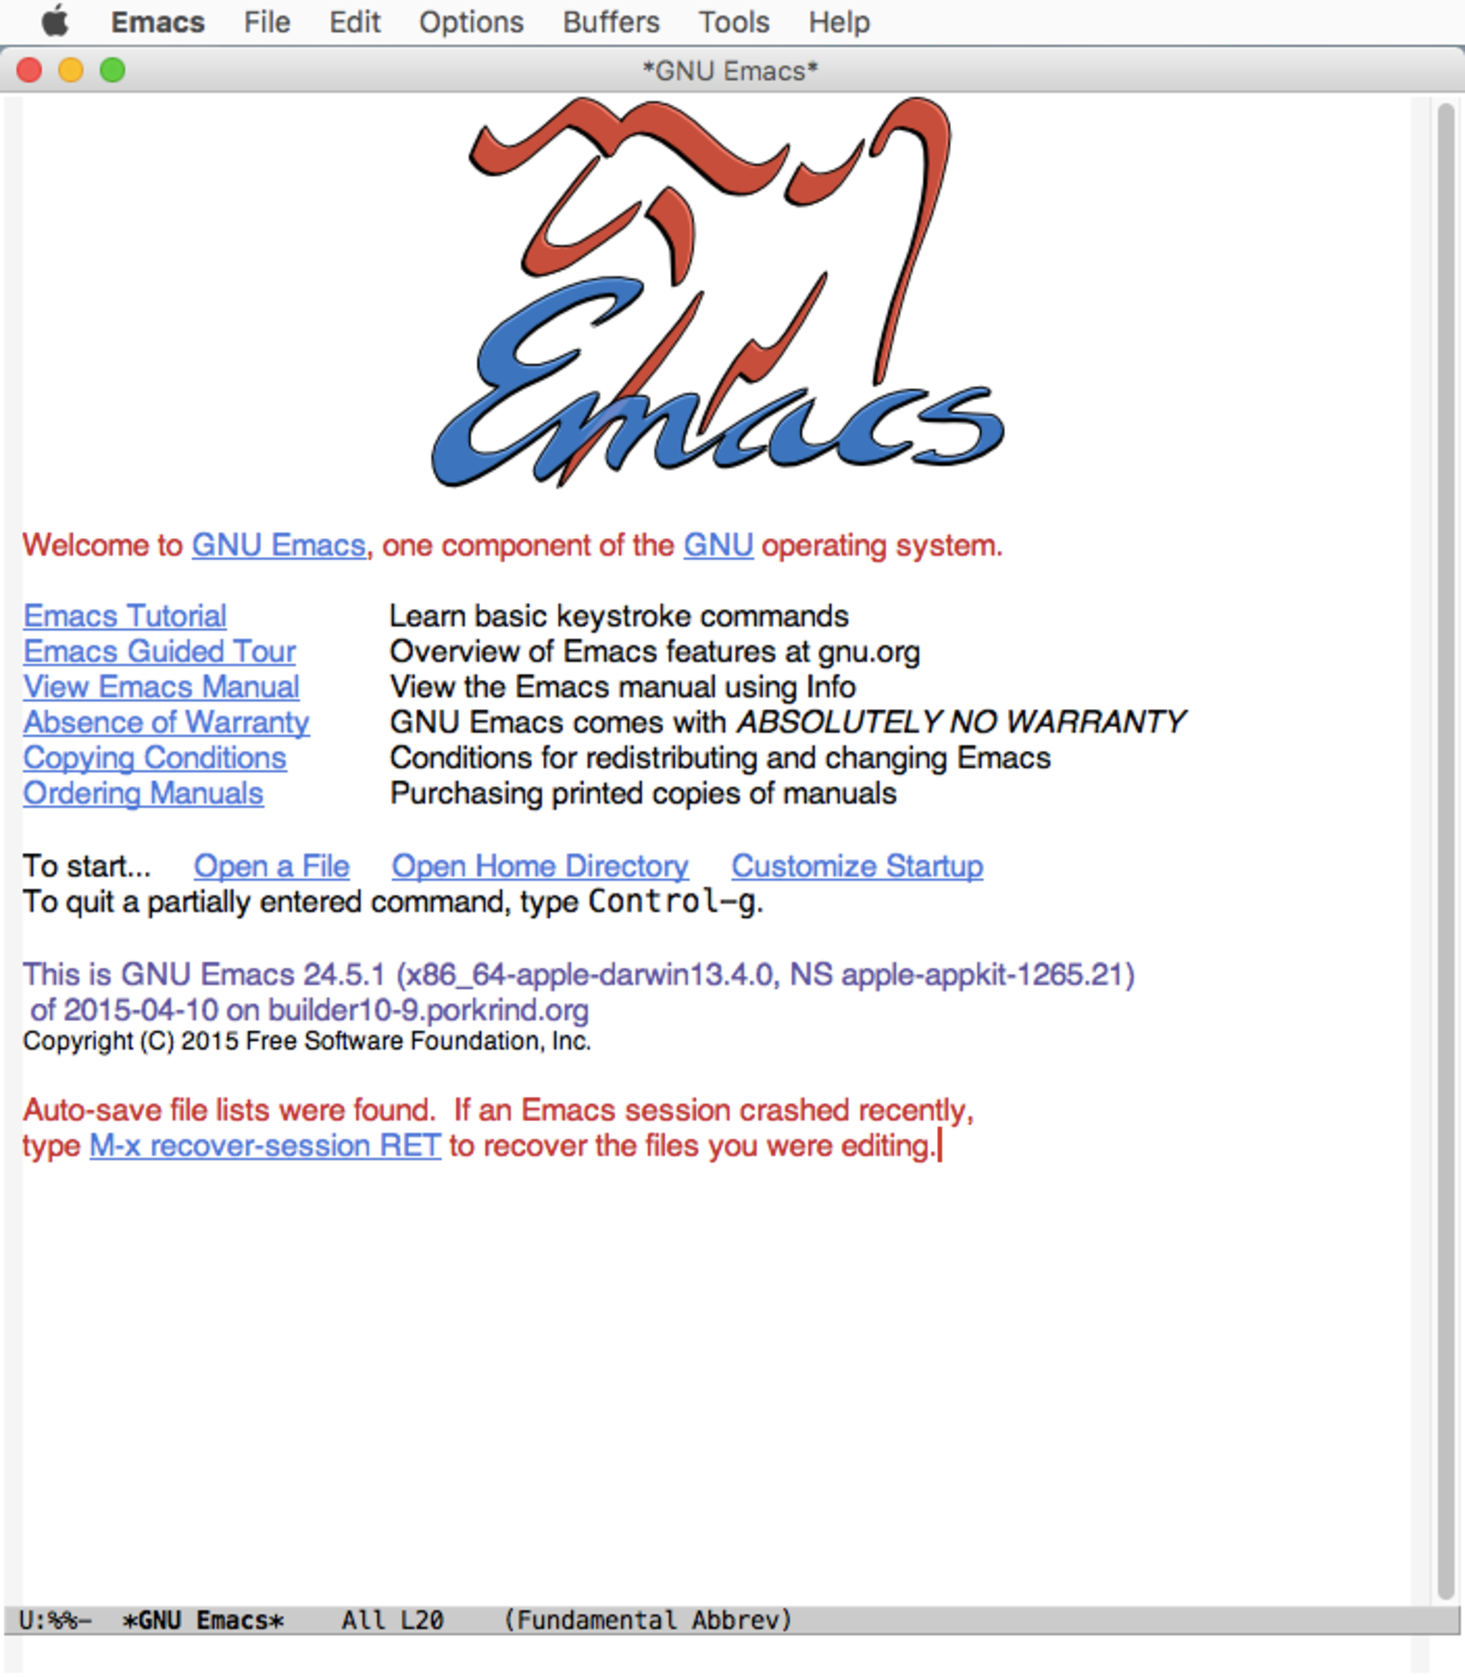
\includegraphics{emacswindow-screenshot}

  %% Identification du minibuffer
  \begin{textblock}{0.35}(7.45,-0.18)
    \LARGE$\leadsto$
  \end{textblock}
  \begin{textblock}{1.75}(7.95,-0.2)
    \small \emph{Minibuffer}
  \end{textblock}

  %% Identification de la barre de menu
  \begin{textblock}{0.35}(7.45,-6.68)
    \LARGE$\leadsto$
  \end{textblock}
  \begin{textblock}{1.75}(7.95,-6.7)
    \small Barre de menu
  \end{textblock}

  %% Identification du buffer
  \begin{textblock}{0.35}(7.45,-3.48)
    \LARGE$\leadsto$
  \end{textblock}
  \begin{textblock}{1.75}(7.95,-3.5)
    \small \emph{Buffer}
  \end{textblock}

  %% Identification de la mode line
  \begin{textblock}{0.35}(7.45,-0.38)
    \LARGE$\leadsto$
  \end{textblock}
  \begin{textblock}{1.75}(7.95,-0.4)
    \small Ligne de mode
  \end{textblock}
  \caption{Fenêtre GNU~Emacs et ses différentes parties au lancement
    de l'application sous Mac OS~X. Sous Windows et Linux, la barre de
    menu se trouve à l'intérieur de la fenêtre.}
  \label{fig:ess:emacswindow}
\end{figure}


\section{\emph{Emacs-ismes} et \emph{Unix-ismes}}
\label{emacs+ess:ismes}

Emacs possède sa propre terminologie qu'il vaut mieux connaître
lorsque l'on consulte la documentation. De plus, l'éditeur fait
siennes certaines conventions du monde Unix et qui sont moins usitées
sur les plateformes Windows et OS~X.

\begin{itemize}
\item Dans les définitions de raccourcis claviers:
  \begin{itemize}
  \item \code{C} est la touche \code{Contrôle} (\ctlkey);
  \item \code{M} est la touche \code{Meta}, qui correspond à la touche
    \code{Alt} de gauche sur un PC ou la touche \code{Option}
    (\optkey) sur un Mac (toutefois, voir l'encadré ci-dessus);
  \item \code{ESC} est la touche \code{Échap} (\esckey) et
    est équivalente à \code{Meta};
  \item \code{SPC} est la barre d'espacement;
  \item \code{DEL} est la touche \code{Retour arrière} (\delkey) ---
    \emph{et non la touche} \code{Supprimer}.
  \item \code{RET} est la touche \code{Entrée} (\returnkey);
  \end{itemize}
\item Toutes les fonctionnalités de Emacs correspondent à une commande
  pouvant être tapée dans le \emph{minibuffer}. \code{M-x} démarre
  l'invite de commande.
\item Le caractère \,\verb=~=\, représente le dossier vers lequel
  pointe la variable d'environnement \code{\$HOME} (Linux, OS~X) ou
  \code{\%HOME\%} (Windows). C'est le dossier par défaut de Emacs.
\item La barre oblique (\code{/}) est utilisée pour séparer les
  dossiers dans les chemins d'accès aux fichiers, même sous Windows.
\item En général, il est possible d'appuyer sur \code{TAB} dans le
  \emph{minibuffer} pour compléter les noms de fichiers ou de
  commandes.
\end{itemize}

\begin{figure}[t]
  \begin{osx}
    Par défaut sous Mac OS~X, la touche \code{Meta} est assignée à
    \code{Option} (\optkey). Sur les claviers français, cela empêche
    d'accéder à certains caractères spéciaux tels que [, ], \{ ou \}.

    Une solution consiste à plutôt assigner la touche \code{Meta} à
    \code{Commande} (\cmdkey). Cela bloque alors l'accès à certains
    raccourcis Mac, mais la situation est moins critique ainsi.

    Pour assigner la touche \code{Meta} à \code{Commande} (\cmdkey) et
    laisser la touche \code{Option} (\optkey) jouer son rôle usuel, il
    suffit d'insérer les lignes suivantes dans son fichier de
    configuration \code{.emacs} (voir la
    \autoref{emacs+ess:configuration}):
\begin{verbatim}
;;; ====================================
;;;  Assigner la touche Meta à Commande
;;;  et laisser Option être Option
;;; ====================================
(setq-default ns-command-modifier 'meta)
(setq-default ns-option-modifier 'none)
\end{verbatim}
  \end{osx}
\end{figure}



\section{Commandes de base}
\label{emacs+ess:commandes}

Emacs comporte une pléthore de commandes, il serait donc futile de
tenter d'en faire une liste exhaustive ici. Nous nous contenterons de
mentionner les commandes les plus importantes regroupées par tâche.

Pour débuter, il est utile de suivre le Tour guidé de Emacs\footnote{%
  \url{http://www.gnu.org/software/emacs/tour/} ou cliquer sur le lien
  dans l'écran d'accueil.} %
et de lire le tutoriel de Emacs, que l'on démarre avec \code{C-h t}.

\subsection{Les essentielles}
\label{emacs+ess:commandes:essentielles}

\begin{ttscript}{M-x}
\item[\emacs{M-x}] démarrer l'invite de commande
\item[\emacs{C-g}] bouton de panique: annuler, quitter! Presser plus
  d'une fois au besoin.
\end{ttscript}

\subsection{Manipulation de fichiers}
\label{emacs+ess:commandes:fichiers}

Entre parenthèses, le nom de la commande Emacs correspondante. On peut
entrer cette commande dans le \emph{minibuffer} au lieu d'utiliser le
raccourci clavier.

\begin{important}
  On remarquera qu'il n'existe pas de commande «nouveau fichier» dans
  Emacs. Pour créer un nouveau fichier, il suffit d'ouvrir un fichier
  n'existant pas.\index{Emacs!nouveau fichier}
\end{important}

\begin{ttscript}{C-x C-w}
  \raggedright
\item[\emacs{C-x C-f}] ouvrir un fichier (\code{find-file})
\item[\emacs{C-x C-s}] sauvegarder
  (\code{save-buffer})\index{Emacs!sauvegarder}
\item[\emacs{C-x C-w}] sauvegarder sous
  (\code{write-file})\index{Emacs!sauvegarder sous}
\item[\emacs{C-x k}] fermer un fichier (\code{kill-buffer})
  \\[\baselineskip]
\item[\emacs{C-\_}] annuler (pratiquement illimité); aussi
  \emacs{C-x u} (\code{undo})
  \\[\baselineskip]
\item[\emacs{C-s}] recherche incrémentale avant
  (\code{isearch-forward})
\item[\emacs{C-r}] Recherche incrémentale arrière
  (\code{isearch-backward})
\item[\emacs{M-\%}] rechercher et remplacer
  (\code{query-replace})\index{Emacs!rechercher et remplacer}
\end{ttscript}


\subsection{Déplacements simples du curseur}
\index{Emacs!déplacement}
\label{emacs+ess:commandes:deplacement}

\begin{ttscript}{C-DEL | C-w}
  \raggedright
\item[\emacs{C-b} | \emacs{C-f}] déplacer d'un caractère vers l'arrière~|~l'avant
  (\code{backward-char} | \code{forward-char})
\item[\emacs{C-a} | \emacs{C-e}] aller au début~|~fin de la ligne
  (\code{move-beginning-of-line} | \code{move-end-of-line})
\item[\emacs{C-p} | \emacs{C-n}] aller à la ligne précédente~|~suivante
  (\code{previous-line} | \code{next-line})
\item[\emacs{M-<} | \emacs{M->}] aller au début~|~fin du fichier
  (\code{beginning-of-buffer} | \code{end-of-buffer}) \\[\baselineskip]
\item[\emacs{DEL} | \emacs{C-d}] effacer le caractère à
  gauche~|~droite du curseur (\code{delete-backward-char} | \code{delete-char})
\item[\emacs{M-DEL} | \emacs{M-d}] effacer le mot à gauche~|~droite
  du curseur (\code{backward-kill-word} | \code{kill-word})
\item[\emacs{C-k}] supprimer jusqu'à la fin de la ligne (\code{kill-line})
\end{ttscript}

\begin{figure}[h]
  \begin{osx}
    Plusieurs des raccourcis clavier de Emacs composés avec la touche
    \code{Contrôle} (\ctlkey) sont valides sous Mac OS~X. Par exemple,
    \ctlkey\,\code{A} et \ctlkey\,\code{E} déplacent le curseur au
    début et à la fin de la ligne dans les champs texte.
  \end{osx}
\end{figure}


\subsection{Sélection de texte, copier, coller, couper}
\index{Emacs!sélection}
\label{emacs+ess:commandes:selection}

\begin{ttscript}{C-x C-w}
  \raggedright
\item[\emacs{C-SPC}] débute la sélection (\code{set-mark-command})
\item[\emacs{C-w}] couper la sélection (\code{kill-region})
\item[\emacs{M-w}] copier la sélection (\code{kill-ring-save})
\item[\emacs{C-y}] coller (\code{yank})
\item[\emacs{M-y}] remplacer le dernier texte collé par la
  sélection précédente (\code{yank-pop})
\end{ttscript}

\begin{itemize}
\item Il est possible d'utiliser les raccourcis clavier usuels de
  Windows (\code{C-c}, \code{C-x}, \code{C-v}) et OS~X
  (\cmdkey\,\code{C}, \cmdkey\,\code{X}, \cmdkey\,\code{V}) en
  activant le mode CUA dans le menu \code{Options}.
\item On peut copier-coller directement avec la souris dans Windows en
  sélectionnant du texte puis en appuyant sur le bouton central (ou la
  molette) à l'endroit souhaité pour y copier le texte.
\end{itemize}


\subsection{Manipulation de fenêtres}
\label{emacs+ess:commandes:fenetres}

\begin{ttscript}{C-x C-w}
\item[\emacs{C-x b}] changer de \emph{buffer}
  (\code{switch-buffer})
\item[\emacs{C-x 2}] séparer l'écran en deux fenêtres
  (\code{split-window-vertically})
\item[\emacs{C-x 1}] conserver uniquement la fenêtre courante
  (\code{delete-other-windows})
\item[\emacs{C-x 0}] fermer la fenêtre courante
  (\code{delete-window})
\item[\emacs{C-x o}] aller vers une autre fenêtre lorsqu'il y en a
  plus d'une (\code{other-window})
\end{ttscript}

\subsection{Manipulation de fichiers de script dans le mode ESS}
\label{emacs+ess:commandes:script}

Dans les versions récentes de ESS (à partir de 12.09 environ), la
manipulation des fichiers de script a été passablement simplifiée par
l'introduction de fonctions «intelligentes» qui s'adaptent à la
situation. Les deux principales commandes à connaître sont les
suivantes:

\begin{ttscript}{C-x C-w}
  \raggedright
\item[\ess{C-RET}] évaluer dans le processus R la ligne sous le
  curseur ou la région sélectionnée, puis déplacer le curseur à la
  prochaine expression (\code{ess-eval-region-or-line-and-step})
\item[\ess{C-c C-c}] évaluer dans le processus R la région sélectionnée, la
  fonction ou le paragraphe dans lequel se trouve le curseur, puis
  déplacer le curseur à la prochaine expression
  (\code{ess-eval-region-or-function-or-paragraph-and-step})
\end{ttscript}
Quelques autres fonctions utiles:
\begin{ttscript}{C-x C-w}
  \raggedright
\item[\ess{C-c C-v}] aide sur une commande R
  (\code{ess-display-help-on-object})
\item[\ess{C-c C-l}] évaluer le code du fichier courant en entier dans
  le processus R (\code{ess-load-file})
\item[\ess{C-c C-n}] évaluer la ligne sous le curseur dans le
  processus R, puis déplacer le curseur à la prochaine expression
  (\code{ess-eval-line-and-step})
\item[\ess{C-c C-r}] évaluer la région sélectionnée dans le processus
  R (\code{ess-eval-region})
\item[\ess{C-c C-f}] évaluer le code de la fonction courante dans
  le processus R (\code{ess-eval-function})
\end{ttscript}

\subsection{Interaction avec l'invite de commande R}
\label{emacs+ess:commandes:invite}

\begin{ttscript}{C-x | C-w}
  \raggedright
\item[\ess{M-p} | \ess{M-n}] commande précédente~|~suivante
  dans l'historique (\code{previous-matching-history-from-input},
  \code{next-matching-history-from-input})
\item[\ess{C-c C-e}] replacer la dernière ligne au bas de la fenêtre
  (\code{comint-show-maximum-output})
\item[\ess{M-h}] sélectionner le résultat de la dernière commande
  (\code{mark-paragraph})
\item[\ess{C-c C-o}] effacer le résultat de la dernière commande
  (\code{comint-delete-output})
\item[\ess{C-c C-v}] aide sur une commande R
  (\code{ess-display-help-on-object})
\item[\ess{C-c C-q}] terminer le processus R (\code{ess-quit})
\end{ttscript}

\subsection{Consultation des rubriques d'aide de R}
\label{emacs+ess:commandes:aide}

\begin{ttscript}{m, m}
  \raggedright
\item[\ess{p} | \ess{n}] aller à la section précédente~|~suivante de
  la rubrique (\code{ess-skip-to-previous-section} |
  \code{ess-skip-to-next-section})
\item[\ess{s a}] aller à la section de la liste des arguments \emph{(Arguments)}
\item[\ess{s D}] aller à la section des détails sur la fonction \emph{(Details)}
\item[\ess{s v}] aller à la section sur la valeur retournée par la
  fonction \emph{(Value)}
\item[\ess{s s}] aller à la section des fonctions apparentée \emph{(See Also)}
\item[\ess{s e}] aller à la section des exemples \emph{(Examples)}
\item[\ess{l}] évaluer la ligne sous le curseur; pratique pour
  exécuter les exemples (\code{ess-eval-line-and-step})
\item[\ess{r}] évaluer la région sélectionnée (\code{ess-eval-region})
\item[\ess{h}] ouvrir une nouvelle rubrique d'aide, par défaut pour le
  mot se trouvant sous le curseur (\code{ess-display-help-on-object})
\item[\ess{q}] retourner au processus ESS en laissant la rubrique
  d'aide visible (\code{ess-switch-to-end-of-ESS})
\item[\ess{x}] fermer la rubrique d'aide et retourner au processus ESS
  (\code{ess-kill-buffer-and-go})
\end{ttscript}



\section{Anatomie d'une session de travail (bis)}
\label{emacs+ess:session}

On reprend ici les étapes d'une \capsule{session de travail} type
présentées à la \autoref{presentation:session}, mais en expliquant
comment compléter chacune dans Emacs avec le mode ESS.

\begin{enumerate}
\item Lancer Emacs et ouvrir un fichier de script avec
  \begin{quote}
    \code{C-x C-f}
  \end{quote}
  ou avec le menu
  \begin{quote}
    \code{File|Open file...}
  \end{quote}
  En spécifiant un nom de fichier qui n'existe pas déjà, on se trouve
  à créer un nouveau fichier de script. S'assurer de terminer le nom
  des nouveaux fichiers par \code{.R} pour que Emacs reconnaisse
  automatiquement qu'il s'agit de fichiers de script R.
\item Démarrer un processus R à l'intérieur même de Emacs avec
  \begin{quote}
    \code{M-x R }\returnkey
  \end{quote}
  Emacs demandera alors de spécifier de répertoire de travail
  (\emph{starting data directory}). Accepter la valeur par défaut, par
  exemple
  \begin{quote}
    \verb=~/ =\returnkey
  \end{quote}
  ou indiquer un autre dossier. Un éventuel message de Emacs à l'effet
  que le fichier \code{.Rhistory} n'a pas été trouvé est sans
  conséquence et peut être ignoré.
\item Composer le code. Lors de cette étape, on se déplacera souvent
  du fichier de script à la ligne de commande afin d'essayer diverses
  expressions. On exécutera également des parties seulement du code se
  trouvant dans le fichier de script. Les commandes les plus utilisées
  sont alors
  \begin{quote}
    \ess{C-RET}\ pour exécuter une ligne du fichier de script; \\
    \ess{C-c C-c}\ pour exécuter un paragraphe du fichier de script; \\
    \emacs{C-x o}\ pour se déplacer d'une fenêtre à l'autre; \\
    \ess{C-c C-e}\ pour replacer la ligne de commande au bas de la
    fenêtre.
  \end{quote}
\item Sauvegarder le fichier de script:
  \begin{quote}
    \emacs{C-x C-s}
  \end{quote}
  Les quatrième et cinquième caractères de la ligne de mode changent
  de \,\verb|**|\, à \,\verb|--|.
\item Sauvegarder si désiré l'espace de travail de R avec
  \code{save.image()}\indexfonction{save.image}. On le répète, cela
  n'est habituellement pas nécessaire à moins que l'espace de travail
  ne contienne des objets importants ou longs à recréer.
\item Quitter le processus R avec
  \begin{quote}
    \ess{C-c C-q}
  \end{quote}
  Cette commande ESS se chargera de fermer tous les fichiers associés
  au processus R. On peut ensuite quitter Emacs en fermant
  l'application de la manière usuelle.
\end{enumerate}



\section{Configuration de l'éditeur}
\index{Emacs!configuration}
\label{emacs+ess:configuration}

Une des grandes forces de Emacs est qu'à peu près chacune de ses
facettes est configurable: couleurs, polices de caractère, raccourcis
clavier, etc.

\begin{itemize}
\item Un utilisateur place ses commandes de configuration dans un
  fichier nommé \code{.emacs} (le point est important!) que Emacs lit
  au démarrage.
\item Le fichier \code{.emacs} doit se trouver dans le dossier
  \,\verb=~/=, c'est-à-dire dans le dossier de départ de l'utilisateur
  sous Linux et OS~X, et dans le dossier référencé par la variable
  d'environnement \code{\%HOME\%} sous Windows.
\end{itemize}


\section{Aide et documentation}
\label{emacs+ess:aide}

Emacs possède son propre système d'aide très exhaustif, mais dont la
navigation est peu intuitive selon les standards d'aujourd'hui.
Consulter le menu \code{Help}.

Autrement, on trouvera les manuels de Emacs et de ESS en divers
formats dans les sites respectifs des deux projets:
\begin{quote}
  \url{http://www.gnu.org/software/emacs} \\
  \url{http://ess.r-project.org}
\end{quote}

Enfin, si le désespoir vous prend au cours d'une séance de codage
intensive, vous pouvez toujours consulter le psychothérapeute Emacs.
On le trouve, bien entendu, dans le menu \code{Help}!

%%% Local Variables:
%%% mode: latex
%%% TeX-master: "introduction_programmation_r"
%%% coding: utf-8
%%% End:
